

\subsection{Implementation}\label{sec:Implementation}

\textit{Author: Keyur Panchal \& Wakeel Khan}

\textbf{Implementation Phase}

In Implementation phase we learn that how team can deliver better apps faster with GitLab Continuous Integration (CI). For instance, if I make a code change to my application and commit it, this will trigger an automatic side pipeline which will build my code and test it. It will also catch potential errors and risk immediately and then we can enable to
communicate to the developer or the creator of that code or where we find an error.

We use the IntelliJ IDEA Integrated Development Environment (IDE) and Visual Studio Code to make a code change and push it to a feature branch. Whenever we do any kind of modification in the application and commit the changes it will be created automatically a new continuous integration pipeline will be triggered. Our pipeline required zero configuration for our side it was automatically configured by GitLab Auto Development and Operations (DevOps) capability.

The pipeline has a few stages and jobs in each stage first it builds and pushes it then it will start a few unit tests and scan jobs that will run in parallel (if any) to speed up the pipeline. We can access each job and see what happens in it when the pipeline run will be finished all test results will be added to the artifacts. You can also download the artifacts of each staging jobs in your local pc to analyze the test result. We can also modify the code in the GitLab web IDE.

We can collaborate with others. Then modified changes which will trigger a new pipeline and will deploy up to staging or production or any other required environment. This developer workflow tells us how each team member can contribute code and push it rapidly to production without introducing new risks or quality issues.

Similarly, we setup a job for unit test cases right after the build job. So, whenever we got a new code changes, it initially goes to the build job which is automatically picked up by GitLab CI pipeline and once build stage is finish its job then it goes to the next stage, which is testing stage. In test stage we perform unit test which is written in Java Junit framework. It has 12 different classes including controller test cases and service test cases and it has 54 different testing methods in total to test each module of java spring boot application. Then we integrate these test cases with the GitLab CI pipeline. Where we are passing detail of these test cases in. When these test cases are done their job then it will create an output. This output we are storing in project's repository in different xml files so, one can see and examine the result of these test cases.

\begin{figure}[htbp]
\centerline{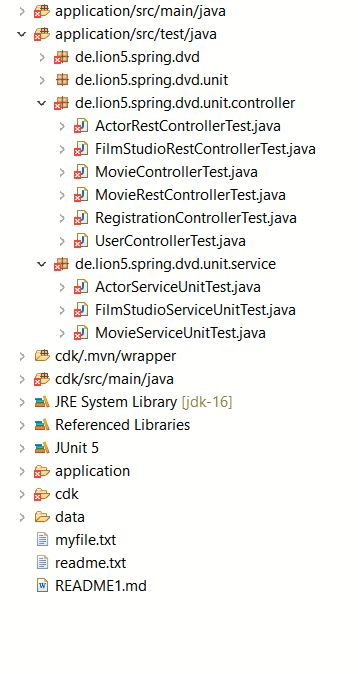
\includegraphics[scale=0.7]{images/keyur_wakeel/Test_Cases_Classes.JPG}}
\label{fig:}
\caption{Test Cases Classes}
\end{figure}

Once our test job is finish then stage goes forward to the next stage job, which is performance. We are performing a load test in this job by using open-source tool JUnit which is very well documented and easy to understand. In this job
our focus is on average response time of our application that how our application handles many users request at a same. This JUnit tool is responsible for measuring the average response time. It creates virtual users and perform Distributed Denial of Service (DDoS) attack (for testing our application performance purpose only).

DDoS stands for Distributed Denial of Service. It is basically a cyber attack on a specific server or network with the aim of disrupting the normal functioning of that network or server. In a DDoS attack, the target network or server is flooded with constant traffic, e.g. with fraudulent requests that overwhelm the system and cause an interruption or
denial of the service of legitimate traffic.

So, we are putting a load of our application to test whether it is performing normal in peak condition or not. If the average response time exceed 500 milliseconds that means our application is not performing well in load condition. So, the pipeline should not be processed further. This is what we implemented in our project. We use JUnit tool to create virtual users to hit our application server and we put a condition if the threshold of http-request-duration average time is greater than 500 milliseconds then failed the test. Otherwise, passed the pipeline and move to the next stage job.


\subsubsection{What is YAML?}

YAML is a serialization language just like Extensible Markup Language (XML) and JavaScript Object Notation (JSON) serialization language basically means that applications written with different technologies languages which have different data structures can transfer data to each other using a common agreed-on or a standard format and the most popular such formats are yaml, json and xml. The name yaml stands for YAML Ain't Markup Language. You can create YAML file with one of those two extensions .yml or .yaml they are the same. YAML define the key value pairs things like variables lists and objects as well.

The main reasons of why YAML popularity has increased so much over the past years is that it is human readable and intuitive which makes it a great fit for writing configuration files for all those recent DevOps tools like docker, Kubernetes etc.

\subsubsection{How is Data Structure Defined?}

In the YAML is through line separations and spaces with indentations that is why wec can indent in space in XML and JSON as we wish, but in the YAML file we will get validation error if we have one single space and data structure wrong which may be a little bit annoying, but it makes YAML format the cleanest most human readable format
of all three.




